We need the Signaling Proxy to translate the information exchange concerning the establishment and control of a communication session. The specific problems related to this component are repeated below:

\begin{itemize}
\item{How to authenticate user identities?}
\item{How to translate the signaling from \gls{wrtc} to Virtual Arena?}
\item{How to handle negotiating the \gls{sdp}?}
\end{itemize}

\section{Authentication}
VA uses Kerberos to authenticate its users, so we need to find a way to do this in the browser somehow. Since we may want users to run a WebRTC application simply by clicking on a link in an email, we need Kerberos to operate with untrusted applications. Normally applications are linked in the Kerberos library, but this would not work for the browser, as it would allow any site the user visits to steal their credentials\cite{webathena}. We may be able to use the Webathena project\footnote{https://github.com/davidben/webathena} created by a MIT student for his master's project\cite{webathena}. The solution consists of a Kerberos client written in Javascript, paired with a server side proxy to wrap the Kerberos protocol in HTTP. We would then be able to delegate credentials to untrusted web applications. I have not been able to test this on VA, so this is a topic for future work.

\section{Signaling}
Since VA has a way of doing signaling that is not relevant for deriving general guidelines, I've chosen to look at more common scenarios. The most used signaling protocol for enterprise communication applications are the SIP protocol. SIP is used to deliver the SDP, which we are required to exchange in WebRTC. \gls{sdp} is an old format used in the \gls{voip} world, therefore the re-use of \gls{sdp} is supposed to save time, but the anatomy of an \gls{sdp} is complex and constantly changing because the \gls{ietf} are coming up with new parameters to include. All the information has to be excactly right or it will be rejected by the browser. It is highly unlikely that the current specification of \gls{sdp} will work with any older implementation found in any enterprise communication system. By using the sipML5 client and the webrtc2sip gateway, I will test to see if we can get a WebRTC application using a SIP stack for Javascript running over WebSockets to interoperate with a desktop SIP client. I tested with a range of different SIP clients to see how well the SIP proxy worked.

\begin{table}[h]
\resizebox{\textwidth}{!}{%
\begin{tabular}{|p{1.3cm}|l|l|p{4cm}|p{4cm}|p{5cm}|}
\hline
SIP desktop clients & Audio & Video  & Perceived delay                                                                                         & Quality                                                  & Comments                                                                                                            \\ \hline
Ekiga               & g.711 & failed & none                                                                                            & good audio quality                                       & did not get video working                                                                                           \\ \hline
Zoiper              & g.711 & vp8    & none for audio, video took approximately 5 seconds to appear, but then it was a live connection & good audio quality, huge packet loss on the video stream & good audio quality, but poor video quality                                                            \\ \hline
Jitsi               & g.711 & failed & none                                                                                            & good audio quality                                       & connection failed every time the application tried to negotiate a video codec, but worked fine when disabling video \\ \hline
Blink               & opus  & failed & none                                                                                            & good audio quality                                       & did not get video working                                                                                           \\ \hline
\end{tabular}
}
\caption{SIP desktop client interaction with web client using proxy and RTCWeb}
\label{tbl:sip-client-webrtc-interaction}
\end{table}

In figure \ref{tbl:sip-client-webrtc-interaction} the audio and video columns refer to the mutually agreed upon codec to be used during the signaling process. Since g.711 is the most preferred codec to be used in \gls{voip} systems, it is natural that audio most often defaults to this codec. Experiments with video conferencing was not very successful. It was difficult getting a normal video session to work for various reasons, one of them being a problem in the \gls{sdp}, which was mentioned earlier as a probable outcome. The one desktop client that did manage to get a working video session using the VP8 codec had a very high packet loss as seen in figure \ref{fig:wireshark-sip-call}. Reasons for this is hard to say as the experiment was done on a really high-bandwidth connection.

\begin{figure}[here]
\centerline{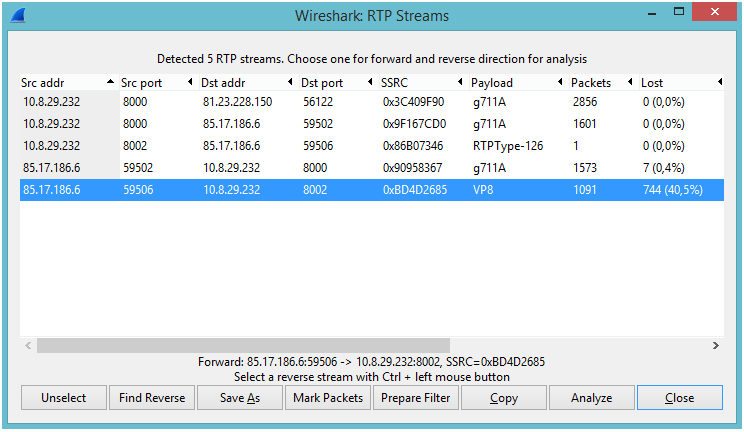
\includegraphics[scale=0.6]{wireshark-rtp.png}}
\caption{Wireshark analysis of a SIP call}
\label{fig:wireshark-sip-call}
\end{figure}

\section{SDP}
In order to get a session going, the most important elements to exchange are the four things (see below) needed for establishing a secure connection, in addition to information about the media:

\begin{itemize}
\item{An ICE username}
\item{An ICE password}
\item{A list of possible ICE candidates}
\item{DTLS fingerprint}s
\end{itemize}

The current \gls{wrtc} specification says to exchange this information with the browser in \gls{sdp} format. But as mentioned earlier it's a bit more complex than that. Here is an example of a failed SDP exchange:

\begin{quote}
Failed to set remote offer sdp: Called with a SDP without crypto enabled. -from WebRTC Internals
\end{quote}

For VA we need to create methods for generating and manipulating the \gls{sdp} in this component.

\section{Summary}
For deriving general guidelines and testing purposes it's easier to envison that our enterprise communication system uses the SIP protocol for signaling purposes rather than VA's proprietary solution. In this chapter we tested the sipML5 client which is essentially a WebRTC client using SIP for signaling. The SIP proxy worked very well for audio, but there was some problems negotiating video, possibly due to different implementations of the SDP, and since SIP is mainly used to deliver the SDP, we should use additional services like the WebAthena proxy to authenticate the users. In the following chapters I will continue to use these experiments as a reference.